\documentclass[crop,border={2pt 2pt 2pt 2pt},tikz]{standalone}
\usepackage{braket}
\usepackage{bbold}
\usepackage{bm}
\usepackage{amsmath}

\usetikzlibrary{backgrounds,decorations.markings, calc}
\tikzset{>=latex}
\tikzset{->-/.style={decoration={
  markings,
  mark=at position .55 with {\arrow{>}}},postaction={decorate}}}
\begin{document}
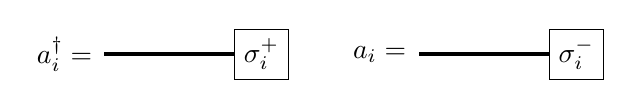
\begin{tikzpicture}

    \coordinate[draw] (i) at (0,0);
    \coordinate[draw] (j) at (3,0);
    

    \node[] at ($(i) + (-2.5, 0)$) {$a^\dagger_i = $};

    \draw[black,very thick] (i) -- +(-2,0); 
   \node[draw,fill = white, anchor = center] at (i) {$\sigma^{+}_i$};

    \begin{scope}[xshift = 4cm ]
        \coordinate[draw] (i) at (0,0);
        \coordinate[draw] (j) at (3,0);
    

        \node[] at ($(i) + (-2.5, 0)$) {$a_i = $};

        \draw[black,very thick] (i) -- +(-2,0); 
        \node[draw,fill = white, anchor = center] at (i) {$\sigma^{-}_i$};
    \end{scope}
   
    

\end{tikzpicture}
\end{document}